\autobookmark
\begin{frame}{Implementation is scalable on cluster systems}
  \begin{columns}

    \begin{column}{.5\textwidth}
        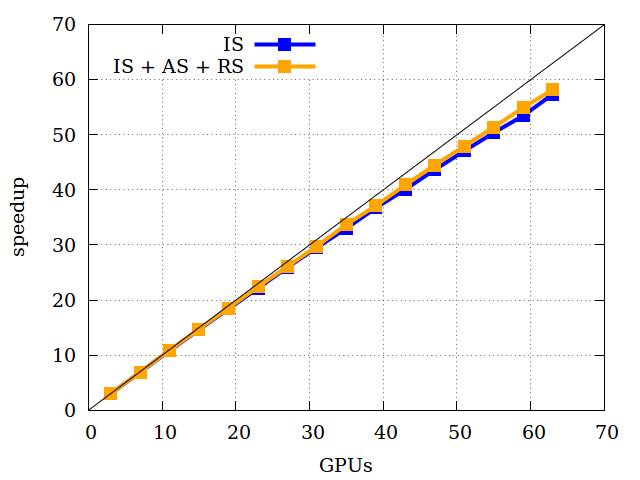
\includegraphics[width=.5\paperwidth]{graphics/scaling.png}
      \end{column}

      \begin{column}{.5\textwidth}
        \begin{itemize}
          \item Load balancing, even when some sample points take longer than others
          \item Implementation scales almost perfectly with an increasing
            number of GPUs in a cluster system
          \item It is possible to simulate even large gain media with high
            precision in a reasonable amount of time
        \end{itemize}
      \end{column}

    \end{columns}
\end{frame}

%\begin{frame}{Predefined colours}
%  The template defines a set of colours according to the CD guidelines:\par
%  \begin{itemize}
%      \begin{minipage}[t]{0.5\linewidth}
%      \item \textcolor{hzdr-blue}{Helmholtz Blue}    
%      \item \textcolor{hzdr-orange}{Rossendorf Orange}  
%      \item \textcolor{hzdr-darkblue}{Helmholtz Dark Blue}
%      \item \textcolor{hzdr-gray1}{Gray1}   
%      \item \textcolor{hzdr-gray2}{Gray2}   
%      \item \textcolor{hzdr-gray3}{Gray3}   
%      \item \textcolor{hzdr-struct}{Structure of Matter}  
%      \end{minipage}%
%      \begin{minipage}[t]{0.5\linewidth}
%      \item \textcolor{hzdr-health}{Health}  
%      \item \textcolor{hzdr-energy}{Energy}  
%      \item \textcolor{hzdr-earth}{Earth and Environment}   
%      \item \textcolor{hzdr-keytec}{Key Technologies}  
%      \item \textcolor{hzdr-aero}{Aeronautics, Space and Transport}
%      \end{minipage}
%  \end{itemize}
%\end{frame}

